\chapter{Tranmission and Distribution}

\section{How to read AC \& DC Schematics and Power System Relaying}
\begin{concept}
    At its core, schematics graphically arrange the components of a system to emphasize the functional arrangement as opposed to the physical arrangement. 
    Emphasizing function facilitates an understanding of how the system is supposed to operate and makes functional testing of systems much easier because it highlights relationships between elements.
\end{concept}

Other names for AC schematics include, AC Elementary Diagrams or Three Line Diagrams. 
DC Schematics are referred to as elementary wiring diagrams. 
The DC schematics depict the DC system and shows the protection and control functions of the equipment in the substation. 
Sometimes the control functions are supplied by AC and are included in the elementary diagram. 
Standards in the AC and DC schematic can differ slightly from utility to utility. 
Both of these schematics will include the rating for circuit elements like resistors, transformers etc.

Any depiction of reality by the single line diagram is on a large scale, it might show where major pieces of equipment are in relation to each other. 
On the other hand, though the AC and DC schematics still don’t show reality in every detail, they will contain information that will provide the link between the real depiction of the equipment seen in wiring diagrams and the almost purely functional depiction shown in the single line diagram.

Another vital function of the AC schematic is to show how the AC current and voltage circuits can be isolated for testing. 
For example, microprocessor delays might contribute to how secondary input quantities are measured as well as the directional sensitivity of specific elements.

\begin{concept}
    \textbf{AC and DC schematics} allow users to quickly trace a signal through the circuit and understand the function without regard to the actual physical wiring locations. 
    Detail will include specific terminal numbers of devices and test switches to which connections are made. 
\end{concept}

\subsection{Common Practices}
\begin{enumerate}
    \item If complexity of the system requires it, the devices controlling the equipment.
    \item The DC circuit is usually shown with the positive bus closer to the top of the page and the negative bus closer to the bottom. 
    The general layout of these drawings is that the DC source is usually shown at the left end of the drawing and the initiating contacts are shown above the operating elements. 
    Control flow is generally shown so that the diagram is read from upper left to lower right.
\end{enumerate}

\subsection{DC Schematics and IEC 61850 Station Bus}
\textbf{DC schematics}: relay systems almost universally use DC for the controls; control ladder diagram or sometimes these are also referred to as elementary wiring diagrams.

IEC 61850 differs from other standards/protocols because it comprises several standards describing client/server and perr-to-peer communications, substation design and configuration, and testing. IEC 61850 provides a method for relay-to-relay interoperability between IEDs from different manufacturers. With the open architecture, it freely supports allocation of C37.2 device functions. The station bus described by IEC 61850 operates digitally over a secure Ethernet based network sending protecting relay messages called Generic Substation Events (GSE) or Generic Object Oriented Substation Events (GOOSE) between relays and other intelligent electronic devices (IEDs) on that network.

Because of this feature, it eliminates most dedicated control wiring that would normally be wired from relay-to-relay (i.e. a trip output contact from one relay to the input coil of another relay). Due to this digital communication between relays, a typical DC schematic diagram alone is not an adequate method for describing the system.

\section{Three-phase Electric Power}
\begin{pline}
    \item \textbf{Three-phase electric power:} a common type of alternating current (AC) used in electricity generation, transmission, and distribution. Typically employs 3-4 wires (fourth wire is an optional neutral return wire).
    \item \textbf{Line voltage:} the voltage between any two lines
    \item \textbf{Phase voltage:} the voltage measured between any line and neutral
\end{pline}
This three-phase electric power is a common method used by electrical grids to transfer power. The voltage on each wire is 120$^\circ$ phase shifted from each other. This allows voltages to be stepped up using transformers to high voltage and stepped down for distribution. Each conductor in a \textit{symmetric} three-phase power supply system carries an alternating current of the same frequency and voltage amplitude. You can design assymetric three-phase power systems, but are not used in practice.

Convention states that for a 208/120-volt service, that means that the line voltage is 208 volts and the phase voltage is 120 volts.

\subsection{Advantages}
If we had to compare a three-phase supply to a single phase AC power supply (with two current-carrying conductors, phase and neutral), a three-phase supply with no neutral and the same phase-to-ground voltage/current capacity per phase would transmit 3 times as much power with only 1.5 imes as much wires (3 vs 2 wires). This means that we get higher efficiency, lower weight, and cleaner waveforms.

Here are more properties of three-phase supplies that are desirable in electric power systems:
\begin{itemize}
    \item Phase currents tend to cancel each other out, summing to 0 in a linear balanced load. Due to this, sometimes we don't even need a neutral conductor since it will carry little or no current.
    \item Power transfer into a linear balanced load is constant, which helps to reduce vibrations in motor/generators
    \item Can produce a rotating magnetic field with a specificed direction and constant magnitude. This simplifies the design of electric motors since no starting circuit is required
\end{itemize}

\subsection{Disadvantages or Cautions}
Make sure that the phases are connected in the correct order to achieve the intended direction of rotation of three-phase motors. If two sources are connected at the same time, then a direct connection between two different phases is a short circuit and leads to flow of unbalanced current.

\subsection{Why not a higher number of phases?}
Three phases is the minumum number that we can have without having "dead" spots in the cycle.

Industry uses almost exclusively three phase power since an induction motor needs at least a three phase supply to start and run in a known direction. Single phase induction motors require lossy, unreliable, and expensive tricks to do the same (extra windings, lossy windings, speed sensitive switch, capacitors, etc).

The supply grid is based on three phase since that is the most efficient in terms of generation and delivery. Using a 9 phase grid for example would require running 9 wires for the entire distribution grid, not cost effective.

The higher order motors mentioned don't use line generated phases. Stepper motors use more phases for finer control. High order polyphase rectifiers are designed often with more 'phases', to reduce ripple, but the phases are generated locally by phase-shifting the line input by some means, either direct LC shifting, or by using a motor-generator set.

Mathematically there is no improvement in motor smoothness, 3 is already an optimal case.

\subsection{Delta and Wye}
There are two basic three-phase configurations
\begin{figure}[H]
    \centering
    \begin{minipage}[c]{0.4\linewidth}
        \centering
        \begin{circuitikz}[american]
            % \tikzset{R/.append style={color=red, /tikz/text=red}}
            \ctikzset{bipoles/resistor/height=0.15}
            \ctikzset{bipoles/resistor/width=0.4}
            \coordinate (A) at (-1,1);
            \coordinate (B) at (0,-1);
            \coordinate (C) at (1,1);
            \coordinate (Rab) at (-0.5,0);
            \coordinate (Rbc) at (0.5,0);
            \coordinate (Rac) at (0,1);
            \draw 
                (A) node[label={left:$A_D$}]{} [R] to  
                (B) node[label={below:$B_D$}]{} [R] to 
                (C) node[label={right:$C_D$}]{} [R] to 
                (A)
                (Rab) node[label={left:$R_{AB}$}]{}
                (Rbc) node[label={right:$R_{BC}$}]{}
                (Rac) node[label={above:$R_{AC}$}]{};
        \end{circuitikz}
        \caption{Delta ($\Delta$) Network}
    \end{minipage}
    \begin{minipage}[c]{0.3\linewidth}
        \centering
        \begin{circuitikz}
        \ctikzset{bipoles/resistor/height=0.15}
            \ctikzset{bipoles/resistor/width=0.4}
            \coordinate (A1) at (-1,1);
            \coordinate (B1) at (0,-1.4);
            \coordinate (C1) at (1,1);
            \coordinate (Ra) at (-0.5,0.5);
            \coordinate (Rb) at (0,-0.5);
            \coordinate (Rc) at (0.5,0.5);
            \coordinate (center) at (0,0);
            \draw
                (A1) node[label={left:A1}]{} [R, *-] to (center)
                (B1) node[label={below:B1}]{} [R, *-] to (center)
                (C1) node[label={right:C1}]{} [R, *-] to (center)
                (Ra) node[label={left:$R_{A}$}]{}
                (Rb) node[label={right:$R_{B}$}]{}
                (Rc) node[label={right:$R_{C}$}]{};
        \end{circuitikz}
        \caption{Wye (Y) Network}
    \end{minipage}
\end{figure}

For a $\wye$ configuration, there is an optional fourth wire, which serves as a neutral and is normally grounded. The ground wire present above many transmission lines are for fault protection and doesn't carry current under normal use.

There are four different types of three-phase transformer winding connections for transmission and distribution.
\begin{pline}
    \item $\wye - \wye$: for small current and high voltage
    \item $\Delta - \Delta$: for large currents and low voltages
    \item $\Delta - \wye$: for step-up transformers (ie generating stations)
    \item $\wye - \Delta$: for step-down transformers (ie at end of the transmission)
\end{pline}

\begin{figure}[H]
    \centering
    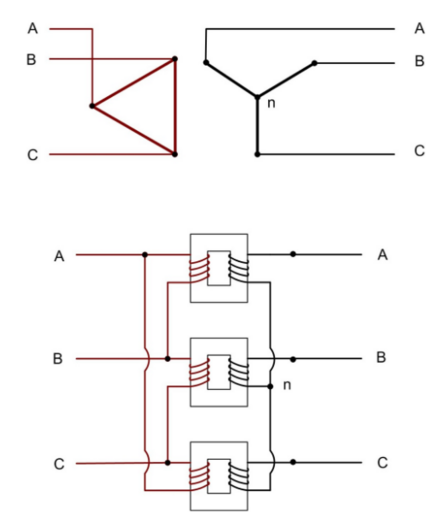
\includegraphics[scale=0.5]{figs/ch03/Delta-Wye_Transformer.png}
    \caption{This shows a delta-wye configuration across a transformer core. A practice transformer wouldn't have a different number of turns on each side.}
\end{figure}

\section{Single-Line Diagrams (SLD)}

\begin{define}
    \textbf{Single-line diagram:} representation of an electrical system, providing a view of its components, interconnections, and electrical flow paths

    \textbf{Bus:} in an electrical system, this is a node where several line or several lines are connected. In power systems specifically, this is any garph node of the single-line diagram at which voltage, curernt, power flow or other quantities can be evaluated
\end{define}
\textbf{More detailed explanation from Schematic Representation of Power System Relaying report:}

Shows the overall scheme and connections and interactions between equipment and relay system components but in a simplified manner. 
For example, it uses a single line to represent three phases (hence the name “single line”). 
The information is shown schematically, but the high- voltage portion is usually shown in a pseudo-physical layout that matches or mimics the actual bus layout in the substation. 
All relays and other major components are assigned a unique identification. 
The identification is carried through the entire drawing set. 
There may be other drawings in the single line format. 
There may also be a one line diagram that emphasizes the power system equipment and does not detail the relay system components but only those elements connected directly at the primary voltage. 
This may be referred to as the “station”, “station one line”, or “power one line” diagram. 
There may also be a simplified one line diagram showing all the protection schemes and their intended zones of protection. 
This is referred to as the “protection zone” or “meter and relay single line” diagram.

\textbf{Components on a single-line diagram}
\begin{pline}
    \item Power sources - includes generators, utility supplies and indicates their voltage levels and connection points to the electrical system
    \item Electrical Equipment - includes transformers, circuit breakers, switches, motors, and loads
    \item Bus arrangement - includes bus bars for power distribution at different voltage levels and shows how power is routed from one location to another
    \item Protective devices - includes fuses, circuit breakers, and relays
    \item Metering/instrumentation - includes metering devices (ammeter, voltmeter etc) and measuring points for monitoring/control
\end{pline}

Bus Arrangement and Voltage Levels
\begin{define}
    Bus duct  
    \begin{itemize}
        \item Carries high currents between different electrical components and sections
        \item Ensures efficient power distribution and reduce
    \end{itemize}
    Transformer 
    \begin{itemize}
        \item Used to step down or setp up voltage levels
        \item Placed at locations to convert high-voltage power from the utility grid to lower voltages or to increase voltage for long-distance Transmission
        \item Winding figurations, type, kVA ratings, cool methods, and surge/lightning protection devices are listed
    \end{itemize}
    Voltage/current transformers (VT, CT)
    \begin{itemize}
        \item Used to measure voltage and current levels for metering, protection, and control purposes
    \end{itemize}
\end{define}

Single line diagrams are the most simplified schematic and least detailed since they rely on basic symbols. We can list a drawing hierarchy from least to most detailed.
\begin{enumerate}
    \item Single line
    \item AC/DC schematics
    \item Logic/wiring diagrams
\end{enumerate}
Each type of schematic has different meaning depending on the intended use. 
Day to day activities associated with power system work include planning, designing, managing, estimating, commissioning, testing, operating, maintaining, consulting, and providing legal records. 
The activities are performed by personnel from different organizational groups such as attorneys, project managers, electricians, relay technicians, design engineers, substation operators, system dispatchers, and system planners. 
How each function is situated within the organizational structure of a power system operator might impact how the different types of drawings are combined and used. 
Certain functions such as real time power system operation have very high priority when compared to activities such as accounting that can be done at any time after the fact. 
This is then reflected into the level of detail contained by each type of drawing depending upon its purposes and priorities.

\subsection{Symbols}
It is difficult to keep a SLD easy to read while including all the necessary data. We want to communicate function using symbols
\begin{figure}[H]
    \centering
    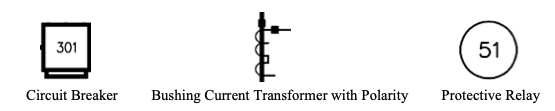
\includegraphics[scale = 0.5]{figs/ch03/sld_symbol.png}
    \caption{Examples of symbols used on one line diagrams}
    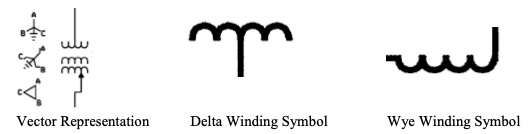
\includegraphics[scale = 0.5]{figs/ch03/sld_3phase.png}
    \caption{Three phase connection in a SLD}
\end{figure}

Guidelines for creating SLDs
\begin{pline}
    \item \textbf{One-Line Representation}: Single-line diagrams use a single line to represent all the electrical components and connections. This helps in reducing complexity and providing a clear overview of the system.
    \item \textbf{Unidirectional Flow}: Electrical power is typically shown to flow from the top of the diagram to the bottom, following a unidirectional flow from the source to the loads.
    \item \textbf{Logical Arrangement}: Components are arranged logically, starting with the power source at the top and then proceeding to the loads at the bottom.
    \item \textbf{Labels and Symbols}: Standardized symbols represent each component uniquely, and labels are used to identify the type and ratings of the equipment.
    \item \textbf{Breakers and Disconnects}: Circuit breakers and disconnect switches are strategically placed to indicate their protective roles and isolation points within the system.
\end{pline}

Circuit Breakers and Protective Devices in Single-Line Diagrams
\begin{itemize}
    \item \textbf{Removeable or Drawout Circuit Breaker}: These circuit breakers can be withdrawn from their housing without disconnecting the electrical connections. 
    They facilitate easy maintenance and replacement of faulty breakers. 
    For instance, a draw-out circuit breaker might protect a critical process in an industrial plant. 
    In case of a fault, the draw-out feature allows quick replacement, minimizing downtime.
    \item \textbf{Non-Drawout Circuit Breaker}: Non-drawout circuit breakers are fixed in their housings and cannot be withdrawn. 
    They are commonly used for less critical circuits or where regular maintenance is not required.
    \item \textbf{Disconnect Switch}: Disconnect switches provide a visible means of isolation and are used to de-energize equipment for maintenance or emergencies. 
    For instance, a disconnect switch might be placed ahead of a motor to isolate it from the power supply during maintenance or repair work.
    \item \textbf{Protective Relays}: Protective relays are connected to current transformers and other sensors to detect abnormal conditions such as overcurrent, undercurrent, or faults. 
    They trigger circuit breakers to open and protect equipment. 
    For instance, a protective relay connected to a current transformer monitors the current flowing to a motor. 
    The relay trips the associated circuit breaker to prevent motor damage if the current exceeds a preset threshold due to a fault.
\end{itemize}

Transformers 
\begin{itemize}
    \item \textbf{Transformer Winding Configurations}: Comes in different windings like $\wye-\wye$
    \item \textbf{Transformer Ratings}: Transformers are rated in kilovolt-amperes (kVA) to indicate their power-carrying capacity. 
    The rating is crucial for determining the transformer's capability and suitability for the application.
    \item \textbf{Cooling Methods}: Transformers can be cooled using different techniques, including natural air convection (KNAN) and forced air cooling (KNAF). 
    The cooling method affects the transformer's thermal performance and is essential for proper sizing and operation.
    \item \textbf{Surge and Lightning Protection}: Surge arresters (metal oxide varistors) are often used to safeguard transformers from voltage surges and lightning strikes. 
    These devices are represented on the SLD and connected to the transformer's incoming terminations.
\end{itemize}

\begin{todo}
    \item resume here
\end{todo}

More symbols loaded below

\includepdf[pages={5,6,7,8,9,10}]{figs/ch03/daltco_wiring_guide}

\section{Sources}
\begin{enumerate}
    \item \href{https://en.wikipedia.org/wiki/Three-phase_electric_power}{Three-phase electric power}: Three phase power section
    \item \href{https://electronics.stackexchange.com/questions/185308/why-three-phase-power-why-not-a-higher-number-of-phases}{Why three-phase power? Why not a higher number of phases?}
    \item \href{https://circuitglobe.com/types-of-faults-in-power-system.html}{Types of Faults in Power System}
    \item AC DC Schematics
    \begin{enumerate}
        \item \href{https://electrical-engineering-portal.com/ac-dc-schematics-protection-control-relaying}{Protection \& Control Relaying Schematics}
        \item \href{https://www.pes-psrc.org/kb/report/047.pdf}{PSRC I5 Schematic Representation of Power System Relaying}
        \item \href{https://www.daltco.com/sites/daltco.com/files/resource/schneider-wiring-diagram-book.pdf}{Wiring diagram book}
        \item \href{https://www.studyforfe.com/blog/fundamentals-of-single-line-diagrams/}{link}
    \end{enumerate}
\end{enumerate}